\documentclass[]{article}
\usepackage{graphicx}
\usepackage{array}
\usepackage{adjustbox}
\usepackage[a4paper,left=1.2cm,right=1.2cm,top=1.4cm,bottom=1.4cm,marginparwidth=2cm]{geometry}

\usepackage{multirow}
\newcommand{\wambsfig}[2]{%
	\includegraphics[page=#1, width=\linewidth, trim=0 0 0 40pt, clip]{#2}%
}

\usepackage{amsmath}
\begin{document}

\begin{center}
	{\Large{\textbf{Matériel et méthodes supplémentaires}}}
\end{center}

Les paramètres sont présentés sur l'échelle logarithmique. Les valeurs obtenues n'ont pas été transformées avec la fonction exponentielle pour les remettre sur leur échelle naturelle.

Les moyennes des paramètres sont arrondies à 3 chiffres significatifs. Les déviations relatives sont calculées à partir des valeurs exactes.

\section{Diamètre myotubes}

\begin{table}[h]
	\centering
	\begin{tabular}{>{\raggedright\arraybackslash}m{2cm}|m{0.13\textwidth}|m{0.10\textwidth}|m{0.15\textwidth}|m{0.20\textwidth}|m{0.18\textwidth}}
		\textbf{Paramètre} & \textbf{Distribution du prior} & \textbf{Type de prior} & \textbf{Source d'information} & \textbf{Plot} & \textbf{Hyperparamètres} \\ \hline
		
		$\beta$ (effet de la condition) & 
		Normale & 
		Faiblement informatif & 
		Absence d'\textit{a priori} directionnel, en autorisant une variation pouvant aller jusqu'à $\approx$ 50\% & 
		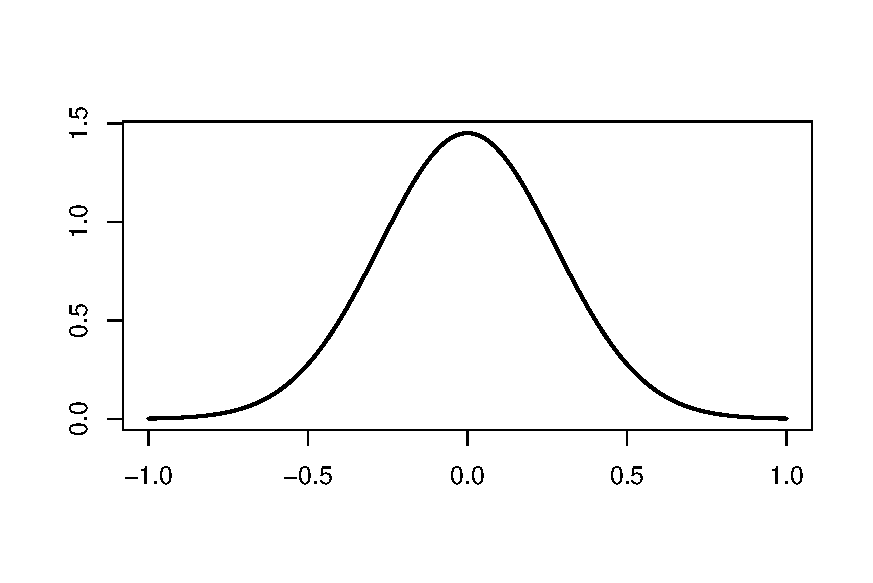
\includegraphics[width=\linewidth]{prior_myotube_beta.pdf} & 
		$\mathcal{N}(0,\ 0.275^2)$ \\
		 
		$\mu_{\alpha}$ (médiane des fibres en BDC-6) & 
		Normale &
		Faiblement informatif & Valeurs crédibles par rapport aux tailles des fibres C2C12
		 & 
		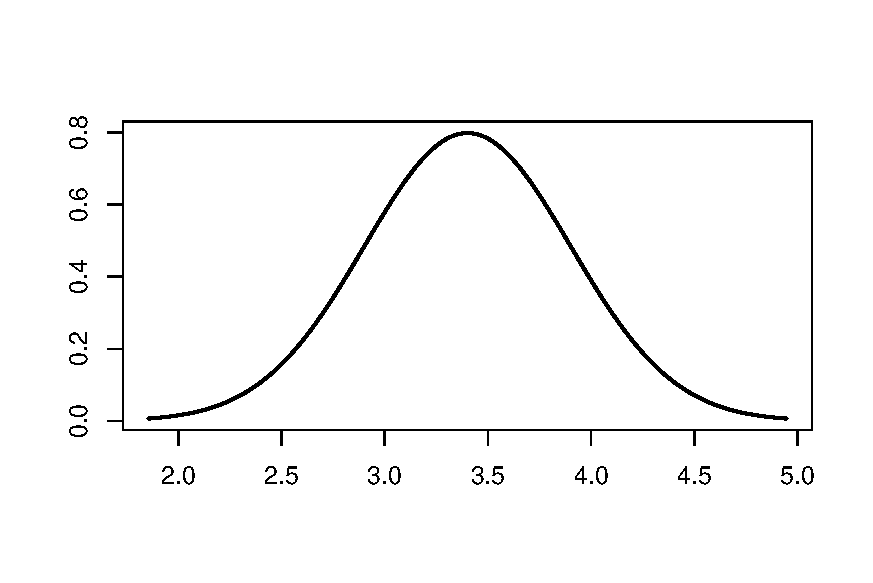
\includegraphics[width=\linewidth]{prior_myotube_mualpha.pdf} & 
		$\mathcal{N}(\ln(30),\ 0.5^2)$ \\
		 
		$\sigma$ (écart-type intra-sujet) &
		Half-Normale &
		Faiblement informatif &
		Recommandations de Gelman et al., 2020 &
		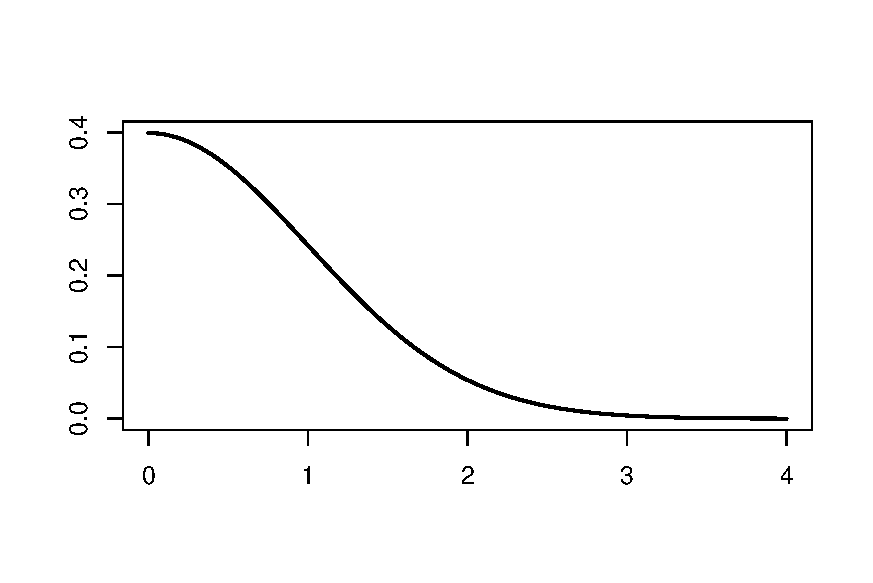
\includegraphics[width=\linewidth]{prior_myotube_sigma.pdf} & 
		$\text{Half-}\mathcal{N}(0, 1)$ \\
		 
		$\sigma$ alpha (écart-type inter-sujets) &
		Half-Normale &
		Faiblement informatif &
		Recommandations de Gelman et al., 2020 &
		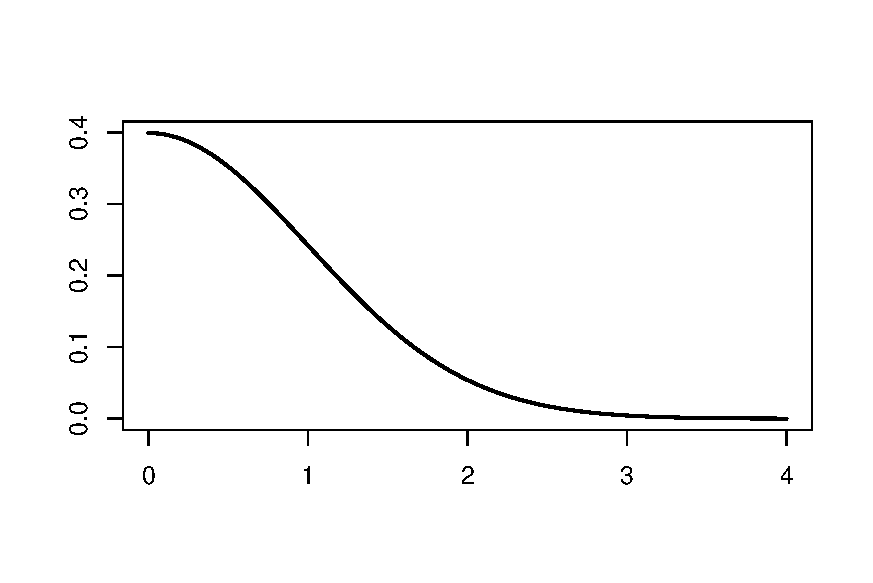
\includegraphics[width=\linewidth]{prior_myotube_sigma.pdf} & 
		 $\text{Half-}\mathcal{N}(0, 1)$ 
	\end{tabular}
	\caption{Do you understand the priors? }
\end{table}

\clearpage

\graphicspath{{wambs_outputs_myotubes/}}

	\begin{table}[h]
		\centering
		
		\begin{adjustbox}{max width=\textwidth}
			
			\begin{tabular}{>{\raggedright\arraybackslash}m{2cm}|m{0.18\textwidth}|m{0.18\textwidth}|m{0.18\textwidth}|m{0.18\textwidth}}
				
				\textbf{Paramètre} & \textbf{Trace plot} & \textbf{Histogramme} & \textbf{Autocorrélation} & \textbf{Density plot} \\
				\hline
				
				$\beta$ (effet de la condition) &
				\wambsfig{1}{base_model.pdf} &
				\wambsfig{2}{base_model.pdf} &
				\wambsfig{3}{base_model.pdf} &
				\wambsfig{4}{base_model.pdf} \\
				
				$\mu_{\alpha}$ (médiane des fibres en BDC-6) &
				\wambsfig{14}{base_model.pdf} &
				\wambsfig{15}{base_model.pdf} &
				\wambsfig{16}{base_model.pdf} &
				\wambsfig{17}{base_model.pdf} \\
				
				$\sigma$ (écart-type intra-sujet) &
				\wambsfig{5}{base_model.pdf} &
				\wambsfig{7}{base_model.pdf} &
				\wambsfig{8}{base_model.pdf} &
				\wambsfig{9}{base_model.pdf} \\
				
				
				$\sigma_{\alpha}$ (écart-type inter-sujets) &
				\wambsfig{10}{base_model.pdf} &
				\wambsfig{11}{base_model.pdf} &
				\wambsfig{12}{base_model.pdf} &
				\wambsfig{13}{base_model.pdf} \\
				
			\end{tabular}
			
		\end{adjustbox}
		
		\caption{WAMBS diagnostics}
	\end{table}

\vspace{2cm}	
	
\begin{table}[h]
	\centering
	
	\begin{adjustbox}{max width=\textwidth}
		
		\begin{tabular}{>{\raggedright\arraybackslash}m{7cm} | >{\raggedright\arraybackslash}m{7cm}}
			
			\textbf{Paramètre} & \textbf{Déviation relative} \\ \hline
			
			Est-ce que la convergence est identique après avoir doublé le nombre d'itérations ? & 
			[(initial converged analysis $-$
			analysis with double
			iterations)/initial converged
			analysis]*100 
			 \\ \hline
			
			\quad $\beta$                                  &  $[(0.014 - 0.014)/0.014] \times 100 = 6\%$\\
			\quad $\mu_{\alpha}$                              &  $[(3.060 - 3.061)/3.060] \times 100 = -0\%$\\
			\quad $\sigma$ (écart-type intra-sujet)        &  $[(0.398 - 0.399)/0.398] \times 100 = -0\%$\\
			\quad $\sigma_{\alpha}$ (écart-type inter-sujets) &  $[(0.019 - 0.019)/0.019] \times 100 = 3\%$ \\ \hline
			
			Est-ce que le prior informatif a un effet notable comparé à un prior non informatif ? & \\ \hline
			
			\quad $\beta$                                  & $[(0.014 - 0.013)/0.014] \times 100 = 7\%$ \\
			\quad $\mu_{\alpha}$                              & $[(3.060 - 3.060)/3.060] \times 100 = 0\%$\\
			\quad $\sigma$ (écart-type intra-sujet)        & $[(0.398 - 0.399)/0.398] \times 100 = -0\%$\\
			\quad $\sigma_{\alpha}$ (écart-type inter-sujets) & $[(0.019 - 0.020)/0.019] \times 100 = -5\%$ \\
			
		\end{tabular}
		
	\end{adjustbox}
	\caption{Effet du prior informatif et du nombre d'itérations}
\end{table}

\clearpage

\begin{table}[h]
	\centering
	
	\begin{adjustbox}{max width=\textwidth}
		
		\begin{tabular}{>{\raggedright\arraybackslash}m{5cm} | >{\raggedright\arraybackslash}m{3cm} | m{3cm} | >{\raggedright\arraybackslash}m{3.6cm}}
			
			\textbf{Comparaison} & \textbf{Mean (sd)} & \textbf{Traceplot} & \textbf{Déviation relative} \\ \hline
			
			\multicolumn{4}{l}{\textit{Comparaison du prior subjectif avec le prior non informatif}} \\ \hline
			
			Prior subjectif $\mathcal{N}(0,\ 0.275^2)$  & 0,014 (0,020) & \wambsfig{1}{base_model.pdf} & \multirow{2}{=}{\raggedright $[(0.014 - 0.013)/0.014] \times 100 = 7\%$} \\
			Prior non informatif $\mathcal{N}(0,\ 5^2)$ & 0,013 (0,020) &\wambsfig{1}{noninf_beta.pdf} & \\ \hline
			
			\multicolumn{4}{l}{\textit{Sensibilité du prior subjectif -- modification des hyperparamètres }} \\ \hline
			
			Comparé à $\mathcal{N}(\ln(1.1),\ 0.275^2)$ & 0,015 (0,020) & \wambsfig{1}{beta_1.pdf} & $[(0.014 - 0.015)/0.014] \times 100 = -5\%$\\
			Comparé à $\mathcal{N}(\ln(1.2),\ 0.275^2)$ & 0,014 (0,020) & \wambsfig{1}{beta_2.pdf} & $[(0.014 - 0.014)/0.014] \times 100 = 1\%$ \\
			Comparé à $\mathcal{N}(\ln(0.9),\ 0.275^2)$ & 0,012 (0,020) & \wambsfig{1}{beta_3.pdf} & $[(0.014 - 0.012)/0.014] \times 100 = 15\%$\\
			Comparé à $\mathcal{N}(\ln(0.8),\ 0.275^2)$ & 0,012 (0,020) & 
			\wambsfig{1}{beta_4.pdf} & $[(0.014 - 0.012)/0.014] \times 100 = 17\%$\\
			
		\end{tabular}
		
	\end{adjustbox}
	\caption{Analyse de la sensibilité du prior pour $\beta$}
\end{table}

\clearpage

\begin{table}[h]
	\centering
	
	\begin{adjustbox}{max width=\textwidth}
		
		\begin{tabular}{>{\raggedright\arraybackslash}m{5cm} | >{\raggedright\arraybackslash}m{3cm} | m{3cm} | >{\raggedright\arraybackslash}m{3.6cm}}
			
			\textbf{Comparaison} & \textbf{Mean (sd)} & \textbf{Traceplot} & \textbf{Déviation relative} \\ \hline
			
			\multicolumn{4}{l}{\textit{Comparaison du prior subjectif avec le prior non informatif}} \\ \hline
			
			Prior subjectif $\mathcal{N}(\ln(30),\ 0.5^2)$  & 3,060 (0,019) & \wambsfig{14}{base_model.pdf} & \multirow{2}{=}{\raggedright $[(3.060 - 3.060)/3.060] \times 100 = 0\%$} \\
			Prior non informatif $\mathcal{N}(0,\ 5^2)$ & 3,060 (0,019) & \wambsfig{14}{noninf_mu.pdf} & \\ \hline
			
			\multicolumn{4}{l}{\textit{Sensibilité du prior subjectif -- modification des hyperparamètres }} \\ \hline
			
			Comparé à $\mathcal{N}(\ln(40),\ 0.5^2)$ & 3,061 (0,027) &\wambsfig{14}{mu_1.pdf} & $[(3.060 - 3.061)/3.060] \times 100 = -0\%$\\
			Comparé à $\mathcal{N}(\ln(50),\ 0.5^2)$ & 3,061 (0,021) & \wambsfig{14}{mu_2.pdf}& $[(3.060 - 3.061)/3.060] \times 100 = -0\%$\\
			Comparé à $\mathcal{N}(\ln(20),\ 0.5^2)$ & 3,060 (0,021) &\wambsfig{14}{mu_3.pdf} & $[(3.060 - 3.060)/3.060] \times 100 = 0\%$\\
			Comparé à $\mathcal{N}(\ln(10),\ 0.5^2)$ & 3,059 (0,020) &\wambsfig{14}{mu_4.pdf} & $[(3.060 - 3.059)/3.060] \times 100 = 0\%$\\
			
		\end{tabular}
		
	\end{adjustbox}
	\caption{Analyse de la sensibilité du prior pour $\mu_{\alpha}$}
	
\end{table}

\clearpage

\begin{figure}[ht]
	\centering
	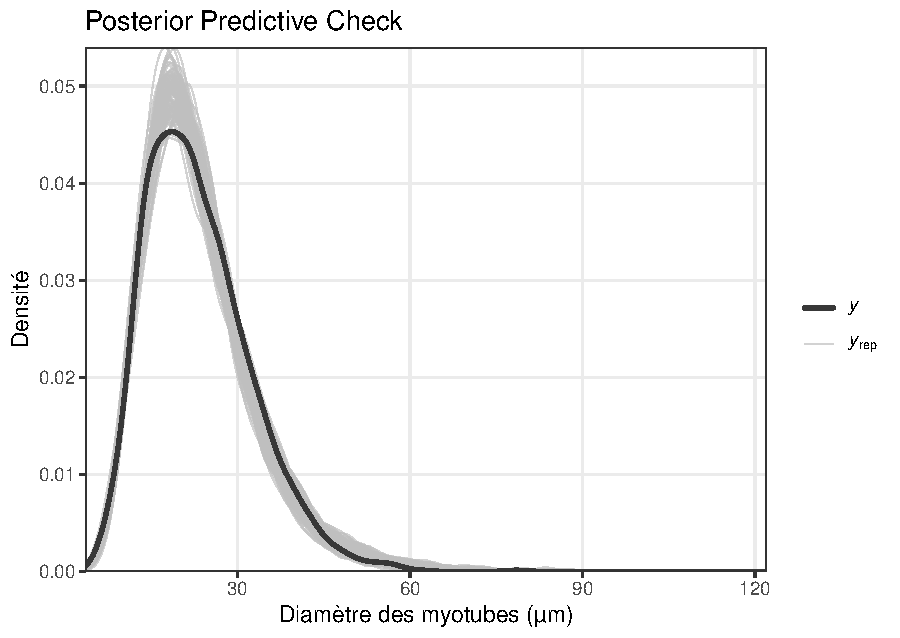
\includegraphics[scale=1]{ppc.pdf}
	\caption{Posterior predictive check de l'analyse du diamètre des myotubes}
\end{figure}

\clearpage

\section{Western blots}

\graphicspath{{}}
\begin{table}[h]
	\centering
	\begin{tabular}{>{\raggedright\arraybackslash}m{2cm}|m{0.13\textwidth}|m{0.10\textwidth}|m{0.15\textwidth}|m{0.20\textwidth}|m{0.18\textwidth}}
		\textbf{Paramètre} & \textbf{Distribution du prior} & \textbf{Type de prior} & \textbf{Source d'information} & \textbf{Plot} & \textbf{Hyperparamètres} \\ \hline
		
		$\beta$ (effet de la condition) & 
		Normale & 
		Faiblement informatif & 
		Absence d'\textit{a priori} directionnel, en autorisant une variation pouvant aller jusqu'à 300\% & 
		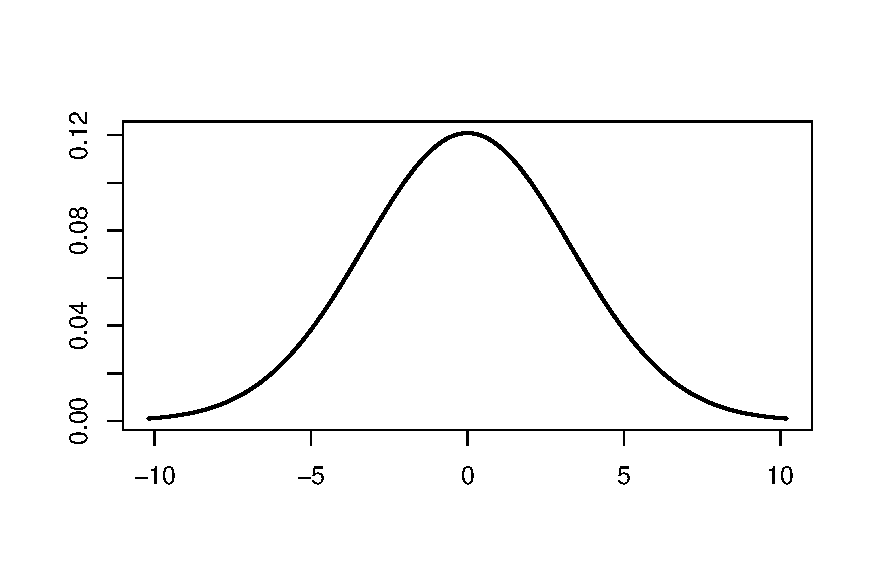
\includegraphics[width=\linewidth]{prior_proteine_beta.pdf} & 
		$\mathcal{N}(0,\ 3.3^2)$ \\
		
		$\sigma$ (écart-type intra-sujet) &
		Half-Normale &
		Faiblement informatif &
		Recommandations de Gelman et al., 2020 &
		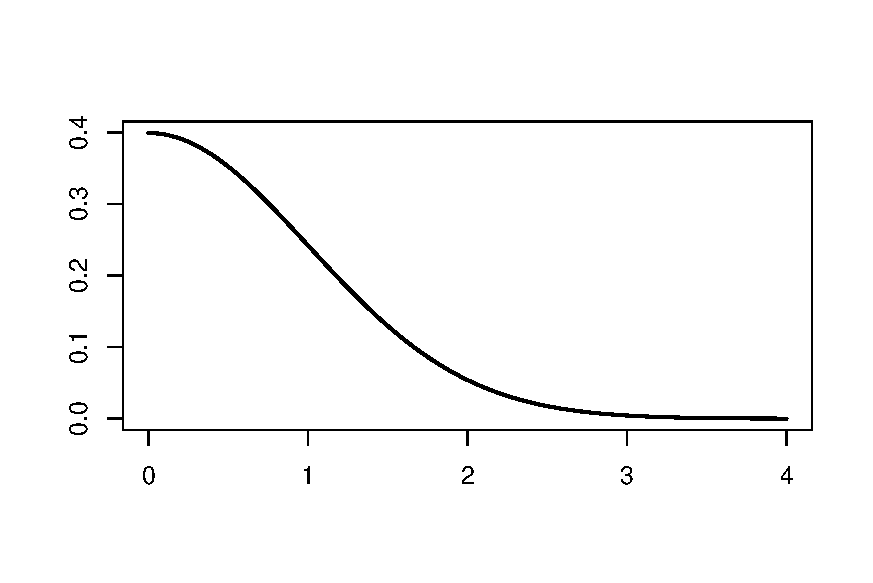
\includegraphics[width=\linewidth]{prior_myotube_sigma.pdf} & 
		$\text{Half-}\mathcal{N}(0, 1)$ \\
		
		$\sigma_{\alpha}$ (écart-type inter-sujets) &
		Half-Normale &
		Faiblement informatif &
		Recommandations de Gelman et al., 2020 &
		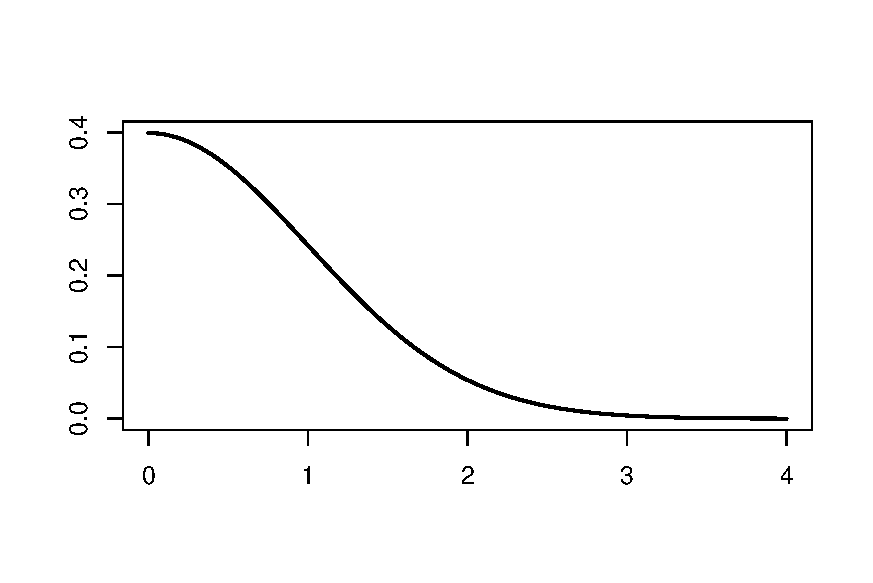
\includegraphics[width=\linewidth]{prior_myotube_sigma.pdf} & 
		$\text{Half-}\mathcal{N}(0, 1)$ 
	\end{tabular}
	\caption{Do you understand the priors? }
\end{table}

\clearpage

\subsection{Myosine}
\graphicspath{{wambs_outputs_proteines/}}

\begin{table}[h]
	\centering
	
	\begin{adjustbox}{max width=\textwidth}
		
		\begin{tabular}{>{\raggedright\arraybackslash}m{2cm}|m{0.18\textwidth}|m{0.18\textwidth}|m{0.18\textwidth}|m{0.18\textwidth}}
			
			\textbf{Paramètre} & \textbf{Trace plot} & \textbf{Histogramme} & \textbf{Autocorrélation} & \textbf{Density plot} \\
			\hline
			
			$\beta$ (effet de la condition) &
			\wambsfig{1}{base_Myosine.pdf} &
			\wambsfig{2}{base_Myosine.pdf} &
			\wambsfig{3}{base_Myosine.pdf} &
			\wambsfig{4}{base_Myosine.pdf} \\
			
			$\sigma$ (écart-type intra-sujet) &
			\wambsfig{5}{base_Myosine.pdf} &
			\wambsfig{7}{base_Myosine.pdf} &
			\wambsfig{8}{base_Myosine.pdf} &
			\wambsfig{9}{base_Myosine.pdf} \\
			
			
			$\sigma_{\alpha}$ (écart-type inter-sujets) &
			\wambsfig{10}{base_Myosine.pdf} &
			\wambsfig{11}{base_Myosine.pdf} &
			\wambsfig{12}{base_Myosine.pdf} &
			\wambsfig{13}{base_Myosine.pdf} \\
			
		\end{tabular}
		
	\end{adjustbox}
	
	\caption{WAMBS diagnostics}
\end{table}

\vspace{2cm}

\begin{table}[h]
	\centering
	
	\begin{adjustbox}{max width=\textwidth}
		
		\begin{tabular}{>{\raggedright\arraybackslash}m{7cm} | >{\raggedright\arraybackslash}m{7cm}}
			
			\textbf{Paramètre} & \textbf{Déviation relative} \\ \hline
			
			Est-ce que la convergence est identique après avoir doublé le nombre d'itérations ? & 
			[(initial converged analysis $-$
			analysis with double
			iterations)/initial converged
			analysis]*100
			\\ \hline
			
			\quad $\beta$                                  &  $[(0.435 - 0.432)/0.435] \times 100 = 1\%$\\
			\quad $\sigma$ (écart-type intra-sujet)        &  $[(0.244 - 0.244)/0.244] \times 100 = -0\%$\\
			\quad $\sigma_{\alpha}$ (écart-type inter-sujets) &  $[(0.291 - 0.284)/0.291] \times 100 = 2\%$ \\ \hline
			
			Est-ce que le prior informatif a un effet notable comparé à un prior non informatif ? & \\ \hline
			
			\quad $\beta$                                  &  $[(0.435 - 0.459)/0.435] \times 100 = -5\%$\\
			\quad $\sigma$ (écart-type intra-sujet)        &  $[(0.244 - 0.241)/0.244] \times 100 = 1\%$\\
			\quad $\sigma_{\alpha}$ (écart-type inter-sujets) &  $[(0.291 - 0.289)/0.291] \times 100 = 1\%$ \\ 
			
		\end{tabular}
		
	\end{adjustbox}
	\caption{Effet du prior informatif et du nombre d'itérations}
\end{table}

\clearpage

\begin{table}[h]
	\centering
	
	\begin{adjustbox}{max width=\textwidth}
		
		\begin{tabular}{>{\raggedright\arraybackslash}m{5cm} | >{\raggedright\arraybackslash}m{3cm} | m{3cm} | >{\raggedright\arraybackslash}m{3.6cm}}
			
			\textbf{Comparaison} & \textbf{Mean (sd)} & \textbf{Traceplot} & \textbf{Déviation relative} \\ \hline
			
			\multicolumn{4}{l}{\textit{Comparaison du prior subjectif avec le prior non informatif}} \\ \hline
			
			Prior subjectif $\mathcal{N}(0,\ 0.55^2)$  & 0,435 (0,133) & \wambsfig{1}{base_Myosine.pdf} & \multirow{2}{=}{\raggedright $[(0.435 - 0.459)/0.435] \times 100 = -5\%$} \\
			Prior non informatif $\mathcal{N}(0,\ 2^2)$ & 0,459 (0,140) &\wambsfig{1}{noninf_beta_Myosine.pdf} & \\ \hline
			
			\multicolumn{4}{l}{\textit{Sensibilité du prior subjectif -- modification des hyperparamètres }} \\ \hline
			
			Comparé à $\mathcal{N}(\ln(2),\ 0.55^2)$ & 0,474 (0,135) & \wambsfig{1}{beta_up_1_Myosine.pdf} & $[(0.435 - 0.474)/0.435] \times 100 = -9\%$\\
			Comparé à $\mathcal{N}(\ln(3),\ 0.55^2)$ & 0,497 (0,135) & \wambsfig{1}{beta_up_2_Myosine.pdf} & $[(0.435 - 0.497)/0.435] \times 100 = -14\%$ \\
			Comparé à $\mathcal{N}(\ln(0.5),\ 0.55^2)$ & 0,387 (0,146) & \wambsfig{1}{beta_down_1_Myosine.pdf} & $[(0.435 - 0.387)/0.435] \times 100 = 11\%$\\
			Comparé à $\mathcal{N}(\ln(0.33),\ 0.55^2)$ & 0,353 (0,166) & 
			\wambsfig{1}{beta_down_2_Myosine.pdf} & $[(0.435 - 0.353)/0.435] \times 100 = 19\%$\\
			
		\end{tabular}
		
	\end{adjustbox}
	\caption{Analyse de la sensibilité du prior pour $\beta$}
\end{table}

\clearpage

\subsection{Ubiquitine}

\begin{table}[h]
	\centering
	
	\begin{adjustbox}{max width=\textwidth}
		
		\begin{tabular}{>{\raggedright\arraybackslash}m{2cm}|m{0.18\textwidth}|m{0.18\textwidth}|m{0.18\textwidth}|m{0.18\textwidth}}
			
			\textbf{Paramètre} & \textbf{Trace plot} & \textbf{Histogramme} & \textbf{Autocorrélation} & \textbf{Density plot} \\
			\hline
			
			$\beta$ (effet de la condition) &
			\wambsfig{1}{base_Ubiquitine.pdf} &
			\wambsfig{2}{base_Ubiquitine.pdf} &
			\wambsfig{3}{base_Ubiquitine.pdf} &
			\wambsfig{4}{base_Ubiquitine.pdf} \\
			
			$\sigma$ (écart-type intra-sujet) &
			\wambsfig{5}{base_Ubiquitine.pdf} &
			\wambsfig{7}{base_Ubiquitine.pdf} &
			\wambsfig{8}{base_Ubiquitine.pdf} &
			\wambsfig{9}{base_Ubiquitine.pdf} \\
			
			
			$\sigma_{\alpha}$ (écart-type inter-sujets) &
			\wambsfig{10}{base_Ubiquitine.pdf} &
			\wambsfig{11}{base_Ubiquitine.pdf} &
			\wambsfig{12}{base_Ubiquitine.pdf} &
			\wambsfig{13}{base_Ubiquitine.pdf} \\
			
		\end{tabular}
		
	\end{adjustbox}
	
	\caption{WAMBS diagnostics}
\end{table}

\vspace{2cm}

\begin{table}[h]
	\centering
	
	\begin{adjustbox}{max width=\textwidth}
		
		\begin{tabular}{>{\raggedright\arraybackslash}m{7cm} | >{\raggedright\arraybackslash}m{7cm}}
			
			\textbf{Paramètre} & \textbf{Déviation relative} \\ \hline
			
			Est-ce que la convergence est identique après avoir doublé le nombre d'itérations ? & 
			[(initial converged analysis $-$
			analysis with double
			iterations)/initial converged
			analysis]*100 
			\\ \hline
			
			\quad $\beta$                                  & $[(-0.054 - -0.048)/-0.054] \times 100 = 11\%$\\
			\quad $\sigma$ (écart-type intra-sujet)        &  $[(0.214 - 0.209)/0.214] \times 100 = 2\%$\\
			\quad $\sigma_{\alpha}$ (écart-type inter-sujets) &  $[(0.134 - 0.149)/0.134] \times 100 = -11\%$ \\ \hline
			
			Est-ce que le prior informatif a un effet notable comparé à un prior non informatif ? & \\ \hline
			
			\quad $\beta$                                  &  $[(-0.054 - -0.055)/-0.054] \times 100 = -3\%$\\
			\quad $\sigma$ (écart-type intra-sujet)        &  $[(0.214 - 0.210)/0.214] \times 100 = 2\%$\\
			\quad $\sigma_{\alpha}$ (écart-type inter-sujets) &  $[(0.134 - 0.152)/0.134] \times 100 = -13\%$ \\ 
			
		\end{tabular}
		
	\end{adjustbox}
	\caption{Effet du prior informatif et du nombre d'itérations}
\end{table}
% 11% d'écart beta après doubler iteration -> mais en vérité différence absolue minime
% Il aurait pu être intéressant de faire avec + d'itération, on est à la limite de la convergence
% + une chaine chez sigma alpha qui n'a pas convergé, peut être lié
\clearpage

\begin{table}[h]
	\centering
	
	\begin{adjustbox}{max width=\textwidth}
		
		\begin{tabular}{>{\raggedright\arraybackslash}m{5cm} | >{\raggedright\arraybackslash}m{3cm} | m{3cm} | >{\raggedright\arraybackslash}m{3.6cm}}
			
			\textbf{Comparaison} & \textbf{Mean (sd)} & \textbf{Traceplot} & \textbf{Déviation relative} \\ \hline
			
			\multicolumn{4}{l}{\textit{Comparaison du prior subjectif avec le prior non informatif}} \\ \hline
			
			Prior subjectif $\mathcal{N}(0,\ 0.55^2)$  & -0.054 (0,108) & \wambsfig{1}{base_Ubiquitine.pdf} & \multirow{2}{=}{\raggedright $[(-0.054 - -0.055)/-0.054] \times 100 = -3\%$} \\
			Prior non informatif $\mathcal{N}(0,\ 2^2)$ & -0.055 (0,110) &\wambsfig{1}{noninf_beta_Ubiquitine.pdf} & \\ \hline
			
			\multicolumn{4}{l}{\textit{Sensibilité du prior subjectif -- modification des hyperparamètres }} \\ \hline
			
			Comparé à $\mathcal{N}(\ln(2),\ 0.55^2)$ & -0,022 (0,111) & \wambsfig{1}{beta_up_1_Ubiquitine.pdf} & $[(-0.054 - -0.022)/-0.054] \times 100 = 60\%$\\
			Comparé à $\mathcal{N}(\ln(3),\ 0.55^2)$ & -0,003 (0,116) & \wambsfig{1}{beta_up_2_Ubiquitine.pdf} & $[(-0.054 - -0.003)/-0.054] \times 100 = 95\%$ \\
			Comparé à $\mathcal{N}(\ln(0.5),\ 0.55^2)$ & -0,076 (0,110) & \wambsfig{1}{beta_down_1_Ubiquitine.pdf} & $[(-0.054 - -0.076)/-0.054] \times 100 = -41\%$\\
			Comparé à $\mathcal{N}(\ln(0.33),\ 0.55^2)$ & -0,092 (0,115) & 
			\wambsfig{1}{beta_down_2_Ubiquitine.pdf} & $[(-0.054 - -0.092)/-0.054] \times 100 = -70\%$\\
			
		\end{tabular}
		
	\end{adjustbox}
	\caption{Analyse de la sensibilité du prior pour $\beta$}
\end{table}

% ECART RELATIF PAS FIABLE pour les petits effets, là on a par ex 95% d'écart mais en vrai en absolu ça bouge quasi pas -> la conclusion serait restée la même

\clearpage

\subsection{P-p38}

\begin{table}[h]
	\centering
	
	\begin{adjustbox}{max width=\textwidth}
		
		\begin{tabular}{>{\raggedright\arraybackslash}m{2cm}|m{0.18\textwidth}|m{0.18\textwidth}|m{0.18\textwidth}|m{0.18\textwidth}}
			
			\textbf{Paramètre} & \textbf{Trace plot} & \textbf{Histogramme} & \textbf{Autocorrélation} & \textbf{Density plot} \\
			\hline
			
			$\beta$ (effet de la condition) &
			\wambsfig{1}{base_P-p38.pdf} &
			\wambsfig{2}{base_P-p38.pdf} &
			\wambsfig{3}{base_P-p38.pdf} &
			\wambsfig{4}{base_P-p38.pdf} \\
			
			$\sigma$ (écart-type intra-sujet) &
			\wambsfig{5}{base_P-p38.pdf} &
			\wambsfig{7}{base_P-p38.pdf} &
			\wambsfig{8}{base_P-p38.pdf} &
			\wambsfig{9}{base_P-p38.pdf} \\
			
			
			$\sigma_{\alpha}$ (écart-type inter-sujets) &
			\wambsfig{10}{base_P-p38.pdf} &
			\wambsfig{11}{base_P-p38.pdf} &
			\wambsfig{12}{base_P-p38.pdf} &
			\wambsfig{13}{base_P-p38.pdf} \\
			
		\end{tabular}
		
	\end{adjustbox}
	
	\caption{WAMBS diagnostics}
\end{table}

\vspace{2cm}

\begin{table}[h]
	\centering
	
	\begin{adjustbox}{max width=\textwidth}
		
		\begin{tabular}{>{\raggedright\arraybackslash}m{7cm} | >{\raggedright\arraybackslash}m{7cm}}
			
			\textbf{Paramètre} & \textbf{Déviation relative} \\ \hline
			
			Est-ce que la convergence est identique après avoir doublé le nombre d'itérations ? & 
			[(initial converged analysis $-$
			analysis with double
			iterations)/initial converged
			analysis]*100
			\\ \hline
			
			\quad $\beta$                                  & $[(-0.097 - -0.096)/-0.097] \times 100 = 2\%$\\
			\quad $\sigma$ (écart-type intra-sujet)        & $[(0.067 - 0.067)/0.067] \times 100 = -1\%$\\
			\quad $\sigma_{\alpha}$ (écart-type inter-sujets) & $[(0.085 - 0.087)/0.085] \times 100 = -2\%$ \\ \hline
			
			Est-ce que le prior informatif a un effet notable comparé à un prior non informatif ? & \\ \hline
			
			\quad $\beta$                                  &  $[(-0.097 - -0.096)/-0.097] \times 100 = 2\%$\\
			\quad $\sigma$ (écart-type intra-sujet)        &  $[(0.067 - 0.068)/0.067] \times 100 = -1\%$\\
			\quad $\sigma_{\alpha}$ (écart-type inter-sujets) &  $[(0.085 - 0.087)/0.085] \times 100 = -2\%$ \\ 
			
		\end{tabular}
		
	\end{adjustbox}
	\caption{Effet du prior informatif et du nombre d'itérations}
\end{table}

\clearpage

\begin{table}[h]
	\centering
	
	\begin{adjustbox}{max width=\textwidth}
		
		\begin{tabular}{>{\raggedright\arraybackslash}m{5cm} | >{\raggedright\arraybackslash}m{3cm} | m{3cm} | >{\raggedright\arraybackslash}m{3.6cm}}
			
			\textbf{Comparaison} & \textbf{Mean (sd)} & \textbf{Traceplot} & \textbf{Déviation relative} \\ \hline
			
			\multicolumn{4}{l}{\textit{Comparaison du prior subjectif avec le prior non informatif}} \\ \hline
			
			Prior subjectif $\mathcal{N}(0,\ 0.55^2)$  & -0.097 (0,038) & \wambsfig{1}{base_P-p38.pdf} & \multirow{2}{=}{\raggedright $[(-0.097 - -0.096)/-0.097] \times 100 = 2\%$} \\
			Prior non informatif $\mathcal{N}(0,\ 2^2)$ & -0.096 (0,040) &\wambsfig{1}{noninf_beta_P-p38.pdf} & \\ \hline
			
			\multicolumn{4}{l}{\textit{Sensibilité du prior subjectif -- modification des hyperparamètres }} \\ \hline
			
			Comparé à $\mathcal{N}(\ln(2),\ 0.55^2)$ & -0,092 (0,040) & \wambsfig{1}{beta_up_1_P-p38.pdf} & $[(-0.097 - -0.092)/-0.097] \times 100 = 6\%$\\
			Comparé à $\mathcal{N}(\ln(3),\ 0.55^2)$ & -0,091 (0,039) & \wambsfig{1}{beta_up_2_P-p38.pdf} & $[(-0.097 - -0.091)/-0.097] \times 100 = 7\%$ \\
			Comparé à $\mathcal{N}(\ln(0.5),\ 0.55^2)$ & -0,100 (0,039) & \wambsfig{1}{beta_down_1_P-p38.pdf} &$[(-0.097 - -0.100)/-0.097] \times 100 = -2\%$\\
			Comparé à $\mathcal{N}(\ln(0.33),\ 0.55^2)$ & -0,102 (0,039) & 
			\wambsfig{1}{beta_down_2_P-p38.pdf} & $[(-0.097 - -0.102)/-0.097] \times 100 = -5\%$\\
			
		\end{tabular}
		
	\end{adjustbox}
	\caption{Analyse de la sensibilité du prior pour $\beta$}
	\end{table}

\clearpage

\subsection{P-AMPK}

\begin{table}[h]
	\centering
	
	\begin{adjustbox}{max width=\textwidth}
		
		\begin{tabular}{>{\raggedright\arraybackslash}m{2cm}|m{0.18\textwidth}|m{0.18\textwidth}|m{0.18\textwidth}|m{0.18\textwidth}}
			
			\textbf{Paramètre} & \textbf{Trace plot} & \textbf{Histogramme} & \textbf{Autocorrélation} & \textbf{Density plot} \\
			\hline
			
			$\beta$ (effet de la condition) &
			\wambsfig{1}{base_P-AMPK.pdf} &
			\wambsfig{2}{base_P-AMPK.pdf} &
			\wambsfig{3}{base_P-AMPK.pdf} &
			\wambsfig{4}{base_P-AMPK.pdf} \\
			
			$\sigma$ (écart-type intra-sujet) &
			\wambsfig{5}{base_P-AMPK.pdf} &
			\wambsfig{7}{base_P-AMPK.pdf} &
			\wambsfig{8}{base_P-AMPK.pdf} &
			\wambsfig{9}{base_P-AMPK.pdf} \\
			
			
			$\sigma_{\alpha}$ (écart-type inter-sujets) &
			\wambsfig{10}{base_P-AMPK.pdf} &
			\wambsfig{11}{base_P-AMPK.pdf} &
			\wambsfig{12}{base_P-AMPK.pdf} &
			\wambsfig{13}{base_P-AMPK.pdf} \\
			
		\end{tabular}
		
	\end{adjustbox}
	
	\caption{WAMBS diagnostics}
\end{table}

\vspace{2cm}

\begin{table}[h]
	\centering
	
	\begin{adjustbox}{max width=\textwidth}
		
		\begin{tabular}{>{\raggedright\arraybackslash}m{7cm} | >{\raggedright\arraybackslash}m{7cm}}
			
			\textbf{Paramètre} & \textbf{Déviation relative} \\ \hline
			
			Est-ce que la convergence est identique après avoir doublé le nombre d'itérations ? & 
			[(initial converged analysis $-$
			analysis with double
			iterations)/initial converged
			analysis]*100
			\\ \hline
			
			\quad $\beta$                                  & $[(0.139 - 0.137)/0.139] \times 100 = 1\%$\\
			\quad $\sigma$ (écart-type intra-sujet)        & $[(0.167 - 0.168)/0.167] \times 100 = -1\%$\\
			\quad $\sigma_{\alpha}$ (écart-type inter-sujets) & $[(0.139 - 0.139)/0.139] \times 100 = -0\%$ \\ \hline
			
			Est-ce que le prior informatif a un effet notable comparé à un prior non informatif ? & \\ \hline
			
			\quad $\beta$                                  &  $[(0.139 - 0.142)/0.139] \times 100 = -2\%$\\
			\quad $\sigma$ (écart-type intra-sujet)        &  $[(0.167 - 0.168)/0.167] \times 100 = -1\%$\\
			\quad $\sigma_{\alpha}$ (écart-type inter-sujets) &  $[(0.139 - 0.142)/0.139] \times 100 = -3\%$ \\ 
			
		\end{tabular}
		
	\end{adjustbox}
	\caption{Effet du prior informatif et du nombre d'itérations}
\end{table}

\clearpage

\begin{table}[h]
	\centering
	
	\begin{adjustbox}{max width=\textwidth}
		
		\begin{tabular}{>{\raggedright\arraybackslash}m{5cm} | >{\raggedright\arraybackslash}m{3cm} | m{3cm} | >{\raggedright\arraybackslash}m{3.6cm}}
			
			\textbf{Comparaison} & \textbf{Mean (sd)} & \textbf{Traceplot} & \textbf{Déviation relative} \\ \hline
			
			\multicolumn{4}{l}{\textit{Comparaison du prior subjectif avec le prior non informatif}} \\ \hline
			
			Prior subjectif $\mathcal{N}(0,\ 0.55^2)$  & 0,139 (0,090) & \wambsfig{1}{base_P-AMPK.pdf} & \multirow{2}{=}{\raggedright $[(0.139 - 0.142)/0.139] \times 100 = -2\%$} \\
			Prior non informatif $\mathcal{N}(0,\ 2^2)$ & 0,142 (0,094) &\wambsfig{1}{noninf_beta_P-AMPK.pdf} & \\ \hline
			
			\multicolumn{4}{l}{\textit{Sensibilité du prior subjectif -- modification des hyperparamètres }} \\ \hline
			
			Comparé à $\mathcal{N}(\ln(2),\ 0.55^2)$ & 0,157 (0,089) & \wambsfig{1}{beta_up_1_P-AMPK.pdf} & $[(0.139 - 0.157)/0.139] \times 100 = -13\%$\\
			Comparé à $\mathcal{N}(\ln(3),\ 0.55^2)$ & 0,168 (0,091) & \wambsfig{1}{beta_up_2_P-AMPK.pdf} & $[(0.139 - 0.168)/0.139] \times 100 = -21\%$ \\
			Comparé à $\mathcal{N}(\ln(0.5),\ 0.55^2)$ & 0,119 (0,089) & \wambsfig{1}{beta_down_1_P-AMPK.pdf} &$[(0.139 - 0.119)/0.139] \times 100 = 14\%$\\
			Comparé à $\mathcal{N}(\ln(0.33),\ 0.55^2)$ & 0,107 (0,092) & 
			\wambsfig{1}{beta_down_2_P-AMPK.pdf} & $[(0.139 - 0.107)/0.139] \times 100 = 23\%$\\
			
		\end{tabular}
		
	\end{adjustbox}
	\caption{Analyse de la sensibilité du prior pour $\beta$}
\end{table}

\clearpage

\subsection{P-Akt}

\begin{table}[h]
	\centering
	
	\begin{adjustbox}{max width=\textwidth}
		
		\begin{tabular}{>{\raggedright\arraybackslash}m{2cm}|m{0.18\textwidth}|m{0.18\textwidth}|m{0.18\textwidth}|m{0.18\textwidth}}
			
			\textbf{Paramètre} & \textbf{Trace plot} & \textbf{Histogramme} & \textbf{Autocorrélation} & \textbf{Density plot} \\
			\hline
			
			$\beta$ (effet de la condition) &
			\wambsfig{1}{base_P-Akt.pdf} &
			\wambsfig{2}{base_P-Akt.pdf} &
			\wambsfig{3}{base_P-Akt.pdf} &
			\wambsfig{4}{base_P-Akt.pdf} \\
			
			$\sigma$ (écart-type intra-sujet) &
			\wambsfig{5}{base_P-Akt.pdf} &
			\wambsfig{7}{base_P-Akt.pdf} &
			\wambsfig{8}{base_P-Akt.pdf} &
			\wambsfig{9}{base_P-Akt.pdf} \\
			
			
			$\sigma_{\alpha}$ (écart-type inter-sujets) &
			\wambsfig{10}{base_P-Akt.pdf} &
			\wambsfig{11}{base_P-Akt.pdf} &
			\wambsfig{12}{base_P-Akt.pdf} &
			\wambsfig{13}{base_P-Akt.pdf} \\
			
		\end{tabular}
		
	\end{adjustbox}
	
	\caption{WAMBS diagnostics}
\end{table}

\vspace{2cm}

\begin{table}[h]
	\centering
	
	\begin{adjustbox}{max width=\textwidth}
		
		\begin{tabular}{>{\raggedright\arraybackslash}m{7cm} | >{\raggedright\arraybackslash}m{7cm}}
			
			\textbf{Paramètre} & \textbf{Déviation relative} \\ \hline
			
			Est-ce que la convergence est identique après avoir doublé le nombre d'itérations ? & 
			[(initial converged analysis $-$
			analysis with double
			iterations)/initial converged
			analysis]*100
			\\ \hline
			
			\quad $\beta$                                  & $[(0.042 - 0.041)/0.042] \times 100 = 4\%$\\
			\quad $\sigma$ (écart-type intra-sujet)        & $[(0.101 - 0.105)/0.101] \times 100 = -4\%$\\
			\quad $\sigma_{\alpha}$ (écart-type inter-sujets) & $[(0.199 - 0.197)/0.199] \times 100 = 1\%$ \\ \hline
			
			Est-ce que le prior informatif a un effet notable comparé à un prior non informatif ? & \\ \hline
			
			\quad $\beta$                                  &  $[(0.042 - 0.041)/0.042] \times 100 = 3\%$\\
			\quad $\sigma$ (écart-type intra-sujet)        &  $[(0.101 - 0.105)/0.101] \times 100 = -4\%$\\
			\quad $\sigma_{\alpha}$ (écart-type inter-sujets) &  $[(0.199 - 0.203)/0.199] \times 100 = -2\%$ \\ 
			
		\end{tabular}
		
	\end{adjustbox}
	\caption{Effet du prior informatif et du nombre d'itérations}
\end{table}

\clearpage

\begin{table}[h]
	\centering
	
	\begin{adjustbox}{max width=\textwidth}
		
		\begin{tabular}{>{\raggedright\arraybackslash}m{5cm} | >{\raggedright\arraybackslash}m{3cm} | m{3cm} | >{\raggedright\arraybackslash}m{3.6cm}}
			
			\textbf{Comparaison} & \textbf{Mean (sd)} & \textbf{Traceplot} & \textbf{Déviation relative} \\ \hline
			
			\multicolumn{4}{l}{\textit{Comparaison du prior subjectif avec le prior non informatif}} \\ \hline
			
			Prior subjectif $\mathcal{N}(0,\ 0.55^2)$  & 0,042 (0,061) & \wambsfig{1}{base_P-Akt.pdf} & \multirow{2}{=}{\raggedright $[(0.042 - 0.041)/0.042] \times 100 = 3\%$} \\
			Prior non informatif $\mathcal{N}(0,\ 2^2)$ & 0,041 (0,067) &\wambsfig{1}{noninf_beta_P-Akt.pdf} & \\ \hline
			
			\multicolumn{4}{l}{\textit{Sensibilité du prior subjectif -- modification des hyperparamètres }} \\ \hline
			
			Comparé à $\mathcal{N}(\ln(2),\ 0.55^2)$ & 0,052 (0,063) & \wambsfig{1}{beta_up_1_P-Akt.pdf} & $[(0.042 - 0.052)/0.042] \times 100 = -24\%$\\
			Comparé à $\mathcal{N}(\ln(3),\ 0.55^2)$ & 0,057 (0,064) & \wambsfig{1}{beta_up_2_P-Akt.pdf} & $[(0.042 - 0.057)/0.042] \times 100 = -33\%$ \\
			Comparé à $\mathcal{N}(\ln(0.5),\ 0.55^2)$ & 0,032 (0,065) & \wambsfig{1}{beta_down_1_P-Akt.pdf} &$[(0.042 - 0.032)/0.042] \times 100 = 25\%$\\
			Comparé à $\mathcal{N}(\ln(0.33),\ 0.55^2)$ & 0,028 (0,065) & 
			\wambsfig{1}{beta_down_2_P-Akt.pdf} & $[(0.042 - 0.028)/0.042] \times 100 = 35\%$\\
			
		\end{tabular}
		
	\end{adjustbox}
	\caption{Analyse de la sensibilité du prior pour $\beta$}
\end{table}

\clearpage

\subsection{P-4EBP1}

\begin{table}[h]
	\centering
	
	\begin{adjustbox}{max width=\textwidth}
		
		\begin{tabular}{>{\raggedright\arraybackslash}m{2cm}|m{0.18\textwidth}|m{0.18\textwidth}|m{0.18\textwidth}|m{0.18\textwidth}}
			
			\textbf{Paramètre} & \textbf{Trace plot} & \textbf{Histogramme} & \textbf{Autocorrélation} & \textbf{Density plot} \\
			\hline
			
			$\beta$ (effet de la condition) &
			\wambsfig{1}{base_P-4EBP1.pdf} &
			\wambsfig{2}{base_P-4EBP1.pdf} &
			\wambsfig{3}{base_P-4EBP1.pdf} &
			\wambsfig{4}{base_P-4EBP1.pdf} \\
			
			$\sigma$ (écart-type intra-sujet) &
			\wambsfig{5}{base_P-4EBP1.pdf} &
			\wambsfig{7}{base_P-4EBP1.pdf} &
			\wambsfig{8}{base_P-4EBP1.pdf} &
			\wambsfig{9}{base_P-4EBP1.pdf} \\
			
			
			$\sigma_{\alpha}$ (écart-type inter-sujets) &
			\wambsfig{10}{base_P-4EBP1.pdf} &
			\wambsfig{11}{base_P-4EBP1.pdf} &
			\wambsfig{12}{base_P-4EBP1.pdf} &
			\wambsfig{13}{base_P-4EBP1.pdf} \\
			
		\end{tabular}
		
	\end{adjustbox}
	
	\caption{WAMBS diagnostics}
\end{table}

\vspace{2cm}

\begin{table}[h]
	\centering
	
	\begin{adjustbox}{max width=\textwidth}
		
		\begin{tabular}{>{\raggedright\arraybackslash}m{7cm} | >{\raggedright\arraybackslash}m{7cm}}
			
			\textbf{Paramètre} & \textbf{Déviation relative} \\ \hline
			
			Est-ce que la convergence est identique après avoir doublé le nombre d'itérations ? & 
			[(initial converged analysis $-$
			analysis with double
			iterations)/initial converged
			analysis]*100
			\\ \hline
			
			\quad $\beta$                                  & $[(-0.053 - -0.053)/-0.053] \times 100 = 0\%$\\
			\quad $\sigma$ (écart-type intra-sujet)        & $[(0.046 - 0.045)/0.046] \times 100 = 2\%$\\
			\quad $\sigma_{\alpha}$ (écart-type inter-sujets) & $[(0.036 - 0.037)/0.036] \times 100 = -3\%$ \\ \hline
			
			Est-ce que le prior informatif a un effet notable comparé à un prior non informatif ? & \\ \hline
			
			\quad $\beta$                                  &  $[(-0.053 - -0.053)/-0.053] \times 100 = -1\%$\\
			\quad $\sigma$ (écart-type intra-sujet)        &  $[(0.046 - 0.045)/0.046] \times 100 = 2\%$\\
			\quad $\sigma_{\alpha}$ (écart-type inter-sujets) &  $[(0.036 - 0.036)/0.036] \times 100 = -1\%$ \\ 
			
		\end{tabular}
		
	\end{adjustbox}
	\caption{Effet du prior informatif et du nombre d'itérations}
\end{table}

\clearpage

\begin{table}[h]
	\centering
	
	\begin{adjustbox}{max width=\textwidth}
		
		\begin{tabular}{>{\raggedright\arraybackslash}m{5cm} | >{\raggedright\arraybackslash}m{3cm} | m{3cm} | >{\raggedright\arraybackslash}m{3.6cm}}
			
			\textbf{Comparaison} & \textbf{Mean (sd)} & \textbf{Traceplot} & \textbf{Déviation relative} \\ \hline
			
			\multicolumn{4}{l}{\textit{Comparaison du prior subjectif avec le prior non informatif}} \\ \hline
			
			Prior subjectif $\mathcal{N}(0,\ 0.55^2)$  & -0,053 (0,025) & \wambsfig{1}{base_P-4EBP1.pdf} & \multirow{2}{=}{\raggedright $[(-0.053 - -0.053)/-0.053] \times 100 = -1\%$} \\
			Prior non informatif $\mathcal{N}(0,\ 2^2)$ & -0,053 (0,025) &\wambsfig{1}{noninf_beta_P-4EBP1.pdf} & \\ \hline
			
			\multicolumn{4}{l}{\textit{Sensibilité du prior subjectif -- modification des hyperparamètres }} \\ \hline
			
			Comparé à $\mathcal{N}(\ln(2),\ 0.55^2)$ & -0,050 (0,024) & \wambsfig{1}{beta_up_1_P-4EBP1.pdf} & $[(-0.053 - -0.050)/-0.053] \times 100 = 4\%$\\
			Comparé à $\mathcal{N}(\ln(3),\ 0.55^2)$ & -0,049 (0,024) & \wambsfig{1}{beta_up_2_P-4EBP1.pdf} & $[(-0.053 - -0.049)/-0.053] \times 100 = 6\%$ \\
			Comparé à $\mathcal{N}(\ln(0.5),\ 0.55^2)$ & -0,055 (0,025) & \wambsfig{1}{beta_down_1_P-4EBP1.pdf} &$[(-0.053 - -0.055)/-0.053] \times 100 = -3\%$\\
			Comparé à $\mathcal{N}(\ln(0.33),\ 0.55^2)$ & -0,054 (0,024) & 
			\wambsfig{1}{beta_down_2_P-4EBP1.pdf} & $[(-0.053 - -0.054)/-0.053] \times 100 = -2\%$\\
			
		\end{tabular}
		
	\end{adjustbox}
	\caption{Analyse de la sensibilité du prior pour $\beta$}
\end{table}

\clearpage

\subsection{P-p70s6k}

\begin{table}[h]
	\centering
	
	\begin{adjustbox}{max width=\textwidth}
		
		\begin{tabular}{>{\raggedright\arraybackslash}m{2cm}|m{0.18\textwidth}|m{0.18\textwidth}|m{0.18\textwidth}|m{0.18\textwidth}}
			
			\textbf{Paramètre} & \textbf{Trace plot} & \textbf{Histogramme} & \textbf{Autocorrélation} & \textbf{Density plot} \\
			\hline
			
			$\beta$ (effet de la condition) &
			\wambsfig{1}{base_P-70s6k.pdf} &
			\wambsfig{2}{base_P-70s6k.pdf} &
			\wambsfig{3}{base_P-70s6k.pdf} &
			\wambsfig{4}{base_P-70s6k.pdf} \\
			
			$\sigma$ (écart-type intra-sujet) &
			\wambsfig{5}{base_P-70s6k.pdf} &
			\wambsfig{7}{base_P-70s6k.pdf} &
			\wambsfig{8}{base_P-70s6k.pdf} &
			\wambsfig{9}{base_P-70s6k.pdf} \\
			
			
			$\sigma_{\alpha}$ (écart-type inter-sujets) &
			\wambsfig{10}{base_P-70s6k.pdf} &
			\wambsfig{11}{base_P-70s6k.pdf} &
			\wambsfig{12}{base_P-70s6k.pdf} &
			\wambsfig{13}{base_P-70s6k.pdf} \\
			
		\end{tabular}
		
	\end{adjustbox}
	
	\caption{WAMBS diagnostics}
\end{table}

\vspace{2cm}

\begin{table}[h]
	\centering
	
	\begin{adjustbox}{max width=\textwidth}
		
		\begin{tabular}{>{\raggedright\arraybackslash}m{7cm} | >{\raggedright\arraybackslash}m{7cm}}
			
			\textbf{Paramètre} & \textbf{Déviation relative} \\ \hline
			
			Est-ce que la convergence est identique après avoir doublé le nombre d'itérations ? & 
			[(initial converged analysis $-$
			analysis with double
			iterations)/initial converged
			analysis]*100
			\\ \hline
			
			\quad $\beta$                                  & $[(-0.158 - -0.160)/-0.158] \times 100 = -1\%$\\
			\quad $\sigma$ (écart-type intra-sujet)        & $[(0.085 - 0.084)/0.085] \times 100 = 0\%$\\
			\quad $\sigma_{\alpha}$ (écart-type inter-sujets) & $[(0.165 - 0.168)/0.165] \times 100 = -2\%$ \\ \hline
			
			Est-ce que le prior informatif a un effet notable comparé à un prior non informatif ? & \\ \hline
			
			\quad $\beta$                                  &  $[(-0.158 - -0.161)/-0.158] \times 100 = -2\%$\\
			\quad $\sigma$ (écart-type intra-sujet)        &  $[(0.085 - 0.085)/0.085] \times 100 = 0\%$\\
			\quad $\sigma_{\alpha}$ (écart-type inter-sujets) &  $[(0.165 - 0.167)/0.165] \times 100 = -1\%$ \\ 
			
		\end{tabular}
		
	\end{adjustbox}
	\caption{Effet du prior informatif et du nombre d'itérations}
\end{table}

\clearpage

\begin{table}[h]
	\centering
	
	\begin{adjustbox}{max width=\textwidth}
		
		\begin{tabular}{>{\raggedright\arraybackslash}m{5cm} | >{\raggedright\arraybackslash}m{3cm} | m{3cm} | >{\raggedright\arraybackslash}m{3.6cm}}
			
			\textbf{Comparaison} & \textbf{Mean (sd)} & \textbf{Traceplot} & \textbf{Déviation relative} \\ \hline
			
			\multicolumn{4}{l}{\textit{Comparaison du prior subjectif avec le prior non informatif}} \\ \hline
			
			Prior subjectif $\mathcal{N}(0,\ 0.55^2)$  & -0,158 (0,051) & \wambsfig{1}{base_P-70s6k.pdf} & \multirow{2}{=}{\raggedright $[(-0.158 - -0.161)/-0.158] \times 100 = -2\%$} \\
			Prior non informatif $\mathcal{N}(0,\ 2^2)$ & -0,161 (0,052) &\wambsfig{1}{noninf_beta_P-70s6k.pdf} & \\ \hline
			
			\multicolumn{4}{l}{\textit{Sensibilité du prior subjectif -- modification des hyperparamètres }} \\ \hline
			
			Comparé à $\mathcal{N}(\ln(2),\ 0.55^2)$ & -0,154 (0,053) & \wambsfig{1}{beta_up_1_P-70s6k.pdf} & $[(-0.158 - -0.154)/-0.158] \times 100 = 3\%$\\
			Comparé à $\mathcal{N}(\ln(3),\ 0.55^2)$ & -0,150 (0,056) & \wambsfig{1}{beta_up_2_P-70s6k.pdf} & $[(-0.158 - -0.150)/-0.158] \times 100 = 5\%$ \\
			Comparé à $\mathcal{N}(\ln(0.5),\ 0.55^2)$ & -0,166 (0,052) & \wambsfig{1}{beta_down_1_P-70s6k.pdf} &$[(-0.158 - -0.166)/-0.158] \times 100 = -5\%$\\
			Comparé à $\mathcal{N}(\ln(0.33),\ 0.55^2)$ & -0,170 (0,055) & 
			\wambsfig{1}{beta_down_2_P-70s6k.pdf} & $[(-0.158 - -0.170)/-0.158] \times 100 = -7\%$\\
			
		\end{tabular}
		
	\end{adjustbox}
	\caption{Analyse de la sensibilité du prior pour $\beta$}
\end{table}

\clearpage

\subsection{PGC1-$\alpha$}


\begin{table}[h]
	\centering
	
	\begin{adjustbox}{max width=\textwidth}
		
		\begin{tabular}{>{\raggedright\arraybackslash}m{2cm}|m{0.18\textwidth}|m{0.18\textwidth}|m{0.18\textwidth}|m{0.18\textwidth}}
			
			\textbf{Paramètre} & \textbf{Trace plot} & \textbf{Histogramme} & \textbf{Autocorrélation} & \textbf{Density plot} \\
			\hline
			
			$\beta$ (effet de la condition) &
			\wambsfig{1}{base_PGC1-alpha.pdf} &
			\wambsfig{2}{base_PGC1-alpha.pdf} &
			\wambsfig{3}{base_PGC1-alpha.pdf} &
			\wambsfig{4}{base_PGC1-alpha.pdf} \\
			
			$\sigma$ (écart-type intra-sujet) &
			\wambsfig{5}{base_PGC1-alpha.pdf} &
			\wambsfig{7}{base_PGC1-alpha.pdf} &
			\wambsfig{8}{base_PGC1-alpha.pdf} &
			\wambsfig{9}{base_PGC1-alpha.pdf} \\
			
			
			$\sigma_{\alpha}$ (écart-type inter-sujets) &
			\wambsfig{10}{base_PGC1-alpha.pdf} &
			\wambsfig{11}{base_PGC1-alpha.pdf} &
			\wambsfig{12}{base_PGC1-alpha.pdf} &
			\wambsfig{13}{base_PGC1-alpha.pdf} \\
			
		\end{tabular}
		
	\end{adjustbox}
	
	\caption{WAMBS diagnostics}
\end{table}

\vspace{2cm}

\begin{table}[h]
	\centering
	
	\begin{adjustbox}{max width=\textwidth}
		
		\begin{tabular}{>{\raggedright\arraybackslash}m{7cm} | >{\raggedright\arraybackslash}m{7cm}}
			
			\textbf{Paramètre} & \textbf{Déviation relative} \\ \hline
			
			Est-ce que la convergence est identique après avoir doublé le nombre d'itérations ? & 
			[(initial converged analysis $-$
			analysis with double
			iterations)/initial converged
			analysis]*100
			\\ \hline
			
			\quad $\beta$                                  & $[(-0.121 - -0.119)/-0.121] \times 100 = 2\%$\\
			\quad $\sigma$ (écart-type intra-sujet)        & $[(0.097 - 0.098)/0.097] \times 100 = -2\%$\\
			\quad $\sigma_{\alpha}$ (écart-type inter-sujets) & $[(0.237 - 0.238)/0.237] \times 100 = -1\%$ \\ \hline
			
			Est-ce que le prior informatif a un effet notable comparé à un prior non informatif ? & \\ \hline
			
			\quad $\beta$                                  &  $[(-0.121 - -0.120)/-0.121] \times 100 = 1\%$\\
			\quad $\sigma$ (écart-type intra-sujet)        &  $[(0.097 - 0.100)/0.097] \times 100 = -3\%$\\
			\quad $\sigma_{\alpha}$ (écart-type inter-sujets) &  $[(0.237 - 0.237)/0.237] \times 100 = -0\%$ \\ 
			
		\end{tabular}
		
	\end{adjustbox}
	\caption{Effet du prior informatif et du nombre d'itérations}
\end{table}

\clearpage

\begin{table}[h]
	\centering
	
	\begin{adjustbox}{max width=\textwidth}
		
		\begin{tabular}{>{\raggedright\arraybackslash}m{5cm} | >{\raggedright\arraybackslash}m{3cm} | m{3cm} | >{\raggedright\arraybackslash}m{3.6cm}}
			
			\textbf{Comparaison} & \textbf{Mean (sd)} & \textbf{Traceplot} & \textbf{Déviation relative} \\ \hline
			
			\multicolumn{4}{l}{\textit{Comparaison du prior subjectif avec le prior non informatif}} \\ \hline
			
			Prior subjectif $\mathcal{N}(0,\ 0.55^2)$  & -0,121 (0,062) & \wambsfig{1}{base_PGC1-alpha.pdf} & \multirow{2}{=}{\raggedright $[(-0.121 - -0.120)/-0.121] \times 100 = 1\%$} \\
			Prior non informatif $\mathcal{N}(0,\ 2^2)$ & -0,120 (0,062) &\wambsfig{1}{noninf_beta_PGC1-alpha.pdf} & \\ \hline
			
			\multicolumn{4}{l}{\textit{Sensibilité du prior subjectif -- modification des hyperparamètres }} \\ \hline
			
			Comparé à $\mathcal{N}(\ln(2),\ 0.55^2)$ & -0,110 (0,064) & \wambsfig{1}{beta_up_1_PGC1-alpha.pdf} & $[(-0.121 - -0.110)/-0.121] \times 100 = 9\%$\\
			Comparé à $\mathcal{N}(\ln(3),\ 0.55^2)$ & -0,108 (0,063) & \wambsfig{1}{beta_up_2_PGC1-alpha.pdf} & $[(-0.121 - -0.108)/-0.121] \times 100 = 11\%$ \\
			Comparé à $\mathcal{N}(\ln(0.5),\ 0.55^2)$ & -0,128 (0,061) & \wambsfig{1}{beta_down_1_PGC1-alpha.pdf} &$[(-0.121 - -0.128)/-0.121] \times 100 = -6\%$\\
			Comparé à $\mathcal{N}(\ln(0.33),\ 0.55^2)$ & -0,135 (0,062) & 
			\wambsfig{1}{beta_down_2_PGC1-alpha.pdf} & $[(-0.121 - -0.135)/-0.121] \times 100 = -11\%$\\
			
		\end{tabular}
		
	\end{adjustbox}
	\caption{Analyse de la sensibilité du prior pour $\beta$}
\end{table}

\clearpage

\begin{figure}[ht]
	\centering
	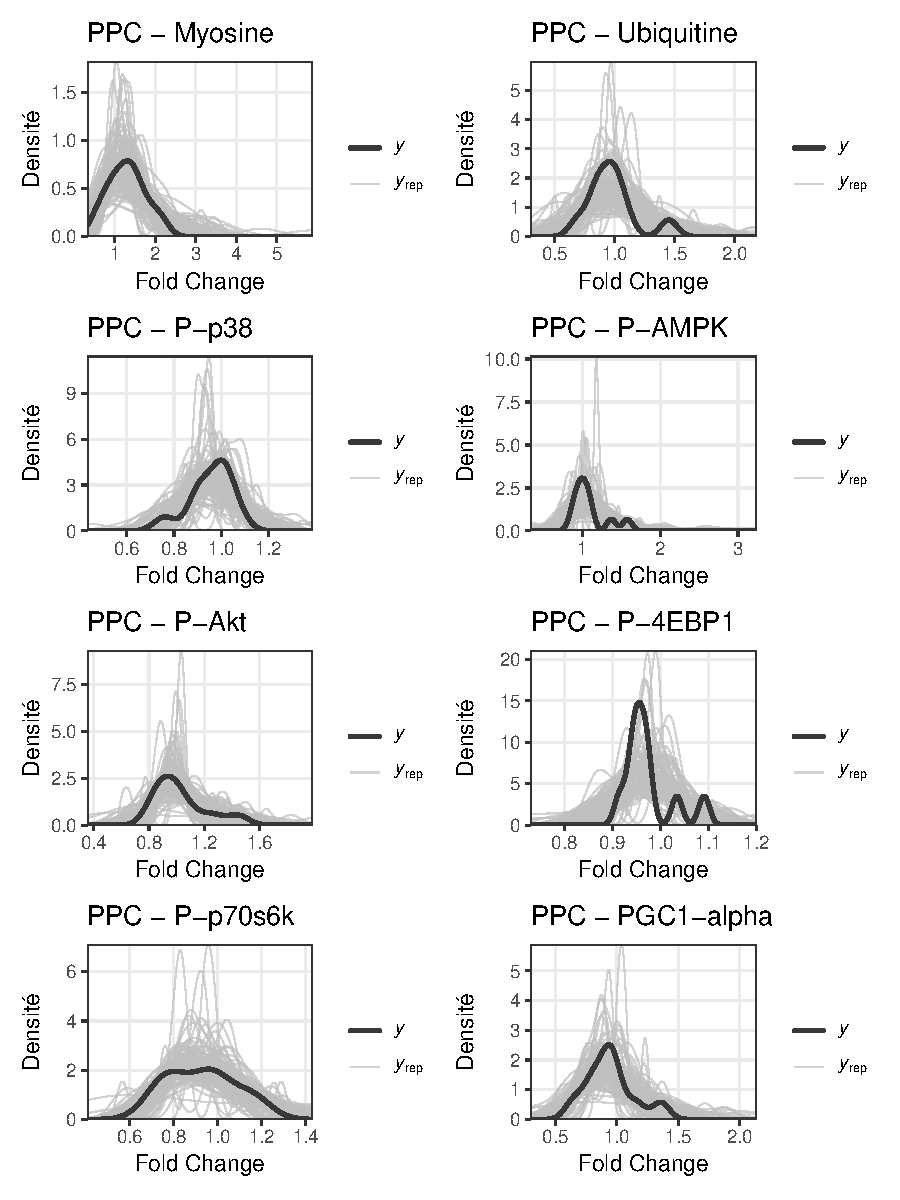
\includegraphics[scale=1.2]{ppc_proteines.pdf}
	\caption{Posterior predictive check de l'analyse de l'expression des protéines d'intérêt}
\end{figure}

\end{document}
